\section{Initialization and Optimization}
\label{sec:imp}
In this section, we summarize the entire framework for our algorithm and then explain how do we initialize the parameters and guide the optimization with input from user interaction for our algorithm.

Based on our formulation in Sec.~\ref{sec:method}, our algorithm can be summarized as in Algorithm \ref{alg:jrcs}.
\begin{algorithm}[htb]
	\caption{Joint Registration and Co-segmentation (JRCS)}
	\label{alg:jrcs}
	\textbf{Input:}~~\\
	$\{\vb{V}_m\}$:$M$ 3D point sets\\
	$\Theta^0$:Initial parameters\\
	$\{\beta_{ik}\}_{m}$:layout based prior\\
	\textbf{Output:}~~\\
	$\Theta^q$:Final parameters~~
	\begin{enumerate}
		\item $q\leftarrow1$
		\item \textbf{repeat}
		\item E-step: Use $\Theta^{q-1}$ to estimate $\alpha_{mik}^q$ according to Eq.~(\ref{equ:estep}) (use Eq.~(\ref{equ:bestep}) for a bilateral formulation);
		\item \textbf{if} $q < q_{alt}$ \textbf{then} Alter $\alpha_{mik}^q$ with $\{\beta_{ik}\}_{m}$ according to Eq.~(\ref{equ:alteralpha});
		\item M-step-a: use $\alpha^q_{mik}$, $\mathbf x^{q-1}_k$ to estimate $\{\mathbf{R}_{mn}^q\}$ and $\{\mathbf t_{mn}^q\}$ according to Eqs.~(\ref{equ:updateR})(\ref{equ:updatet});
		\item M-step-b: use $\alpha^q_{mik}$, $\{\mathbf{R}_{mn}^q\}$ and $\{\mathbf{t}_{mn}^q\}$ to update other parameters for Gaussian models according to Eqs.~ (\ref{equ:updatexk})(\ref{equ:updatesigma})(\ref{equ:updatepk})(\ref{equ:updatey})  (or use Eqs.~ (\ref{equ:updatefk})(\ref{equ:updatefsigma}) for a bilateral formulation);
		\item $q \leftarrow q+1$
		\item \textbf{until} $q > q_{max}$
		\item \textbf{return} $\Theta^q$
	\end{enumerate}
\end{algorithm}
\subsection{Initialization}
\label{sec:imp:interact}
Unfortunately, there are a large number of parameters that can not be easily initialized in our formulation. We let users to place boxes in one of the point sets to help with the initialization, as shown in Figure~\ref{fig:interact}. In this interaction, user can use boxes with different colors to indicate a scene layout for different objects in one of the point sets.\\
In following paragraphs, we explain how we can initialize the parameters in our formulation with these boxes.

\noindent\textbf{Number of objects $N$:} we can naturally determine the $N$ as the number of different color label of the boxes.
 
\noindent\textbf{Number of Gaussian models in each object $\{K_n\}_N$:} The $K_n$ can be set as (\ref{equ:K_n}): 
\begin{equation}
\label{equ:K_n}
K_n=\frac{V_n}{\sum V_n}K_{all}
\end{equation}
in which the $V_n$ represent the total volume of the boxes in the $n^{th}$ color and the $K_{all}$ is initialized as $K_{all}=\frac{median(L_m)}{2}$ and $\{L_m\}_M$ are point numbers of $M$ input point sets. This is an empirical choice borrowed from \cite{Evangelidis2014}.
\begin{figure}
	\centering
	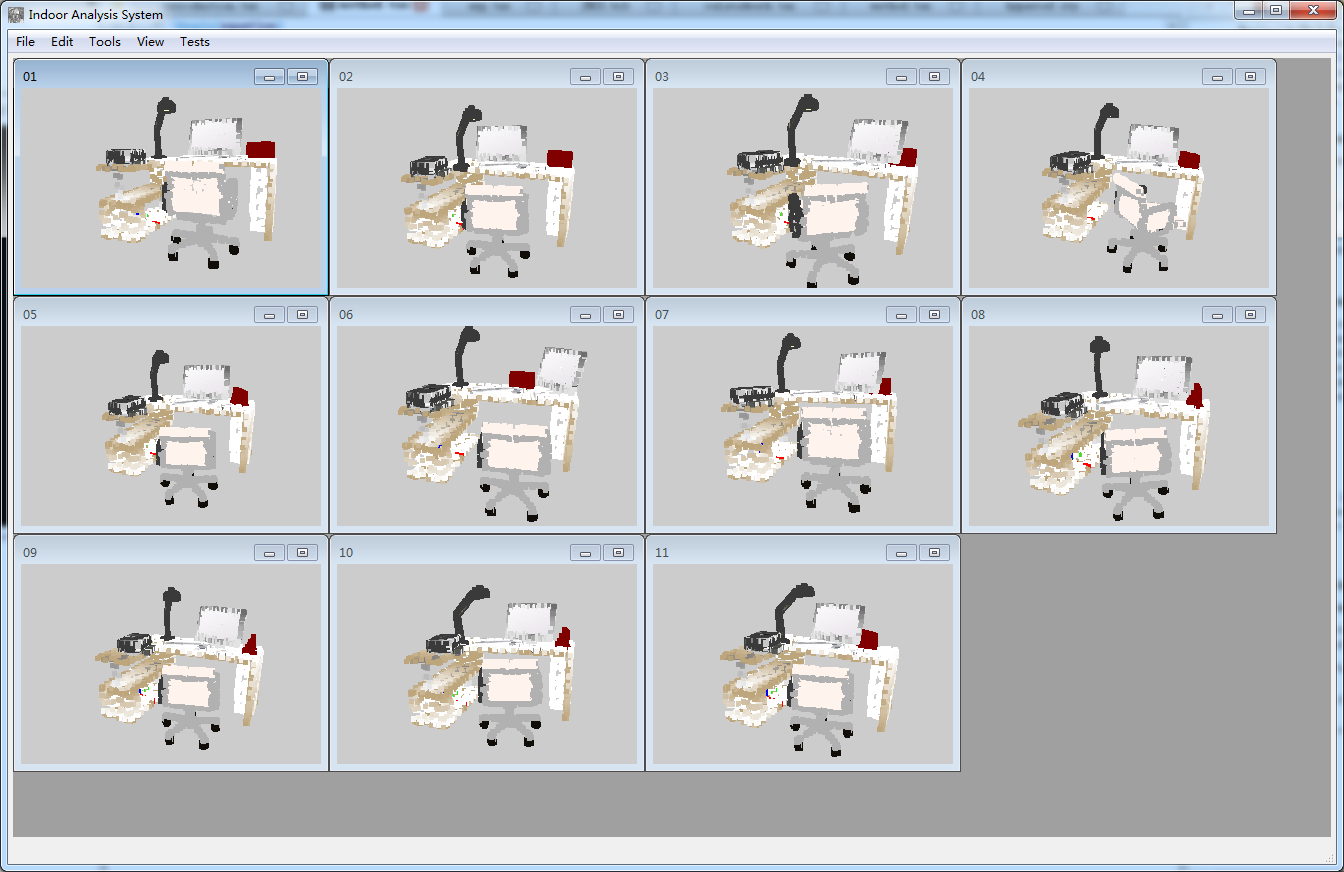
\includegraphics[width=.3\linewidth]{images/interact01.png}
	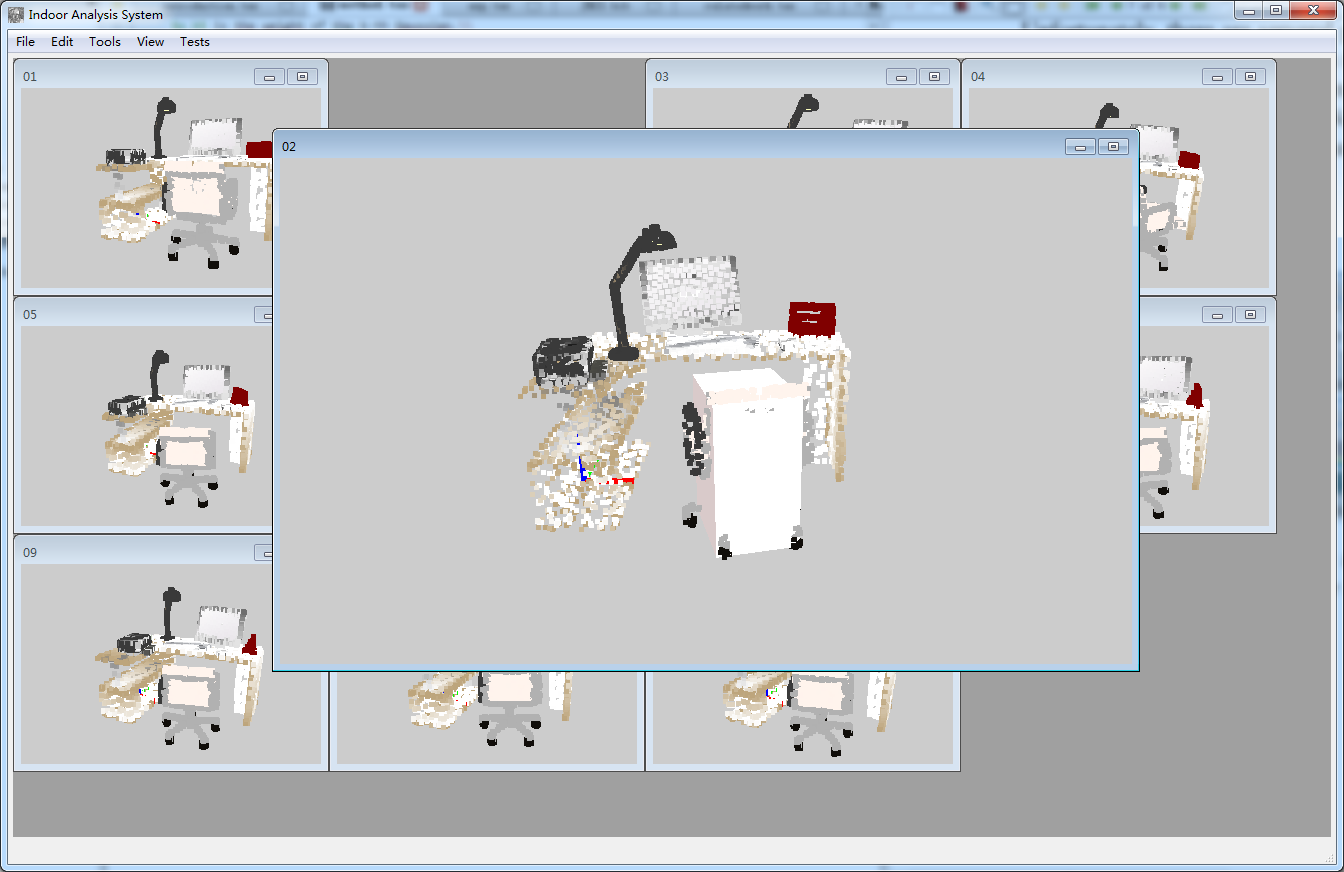
\includegraphics[width=.3\linewidth]{images/interact02.png}
	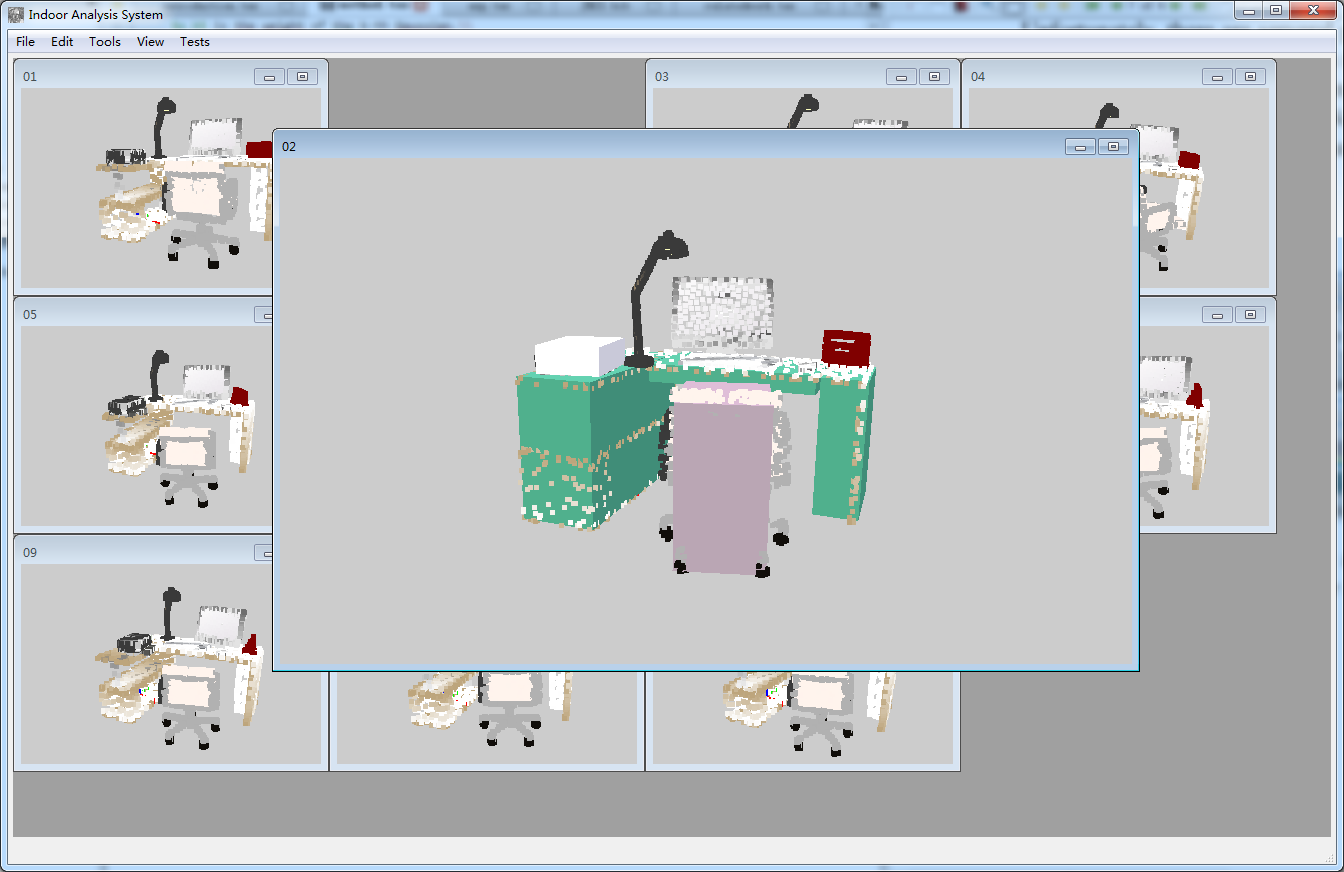
\includegraphics[width=.3\linewidth]{images/interact03.png}
	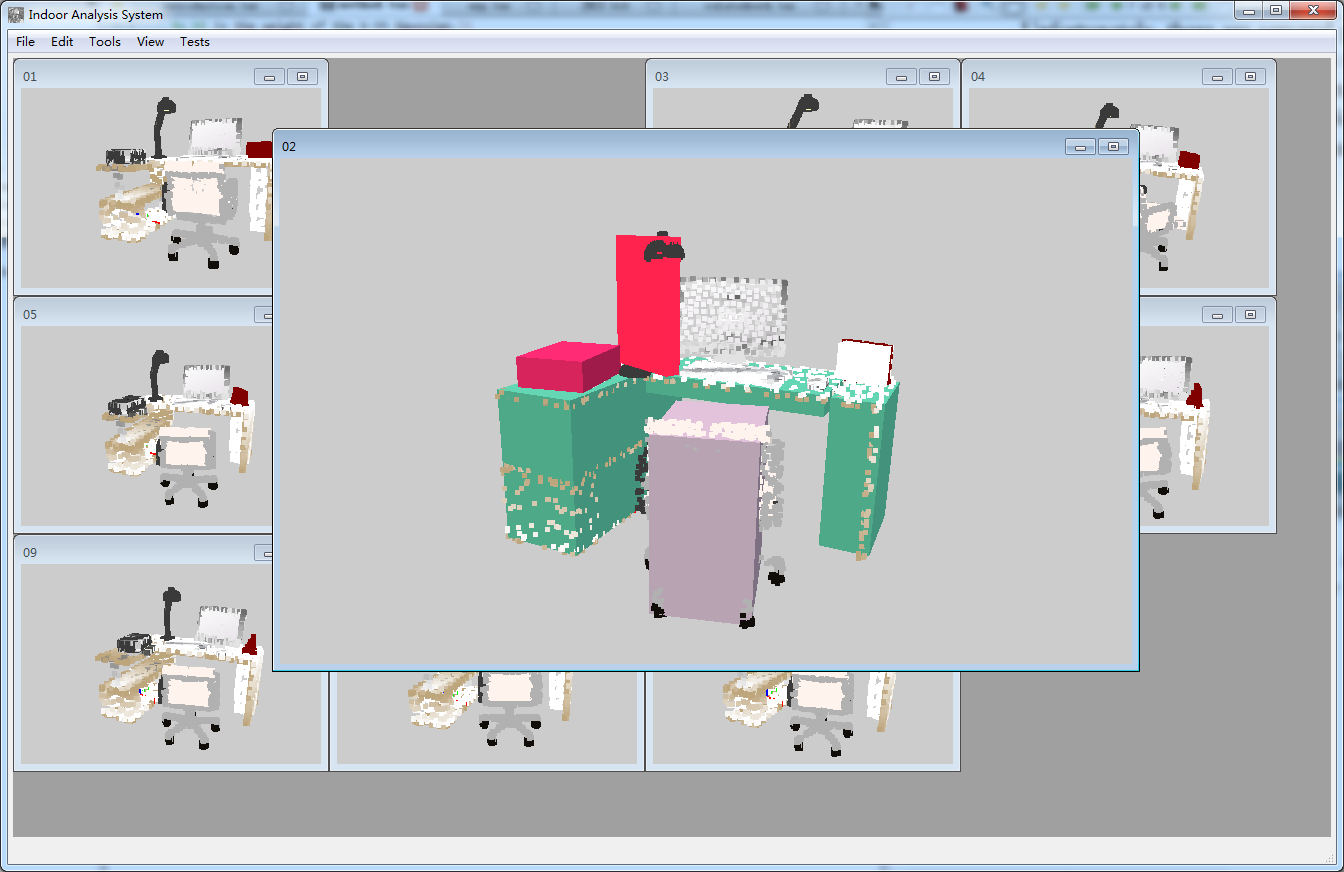
\includegraphics[width=.3\linewidth]{images/interact04.png}
	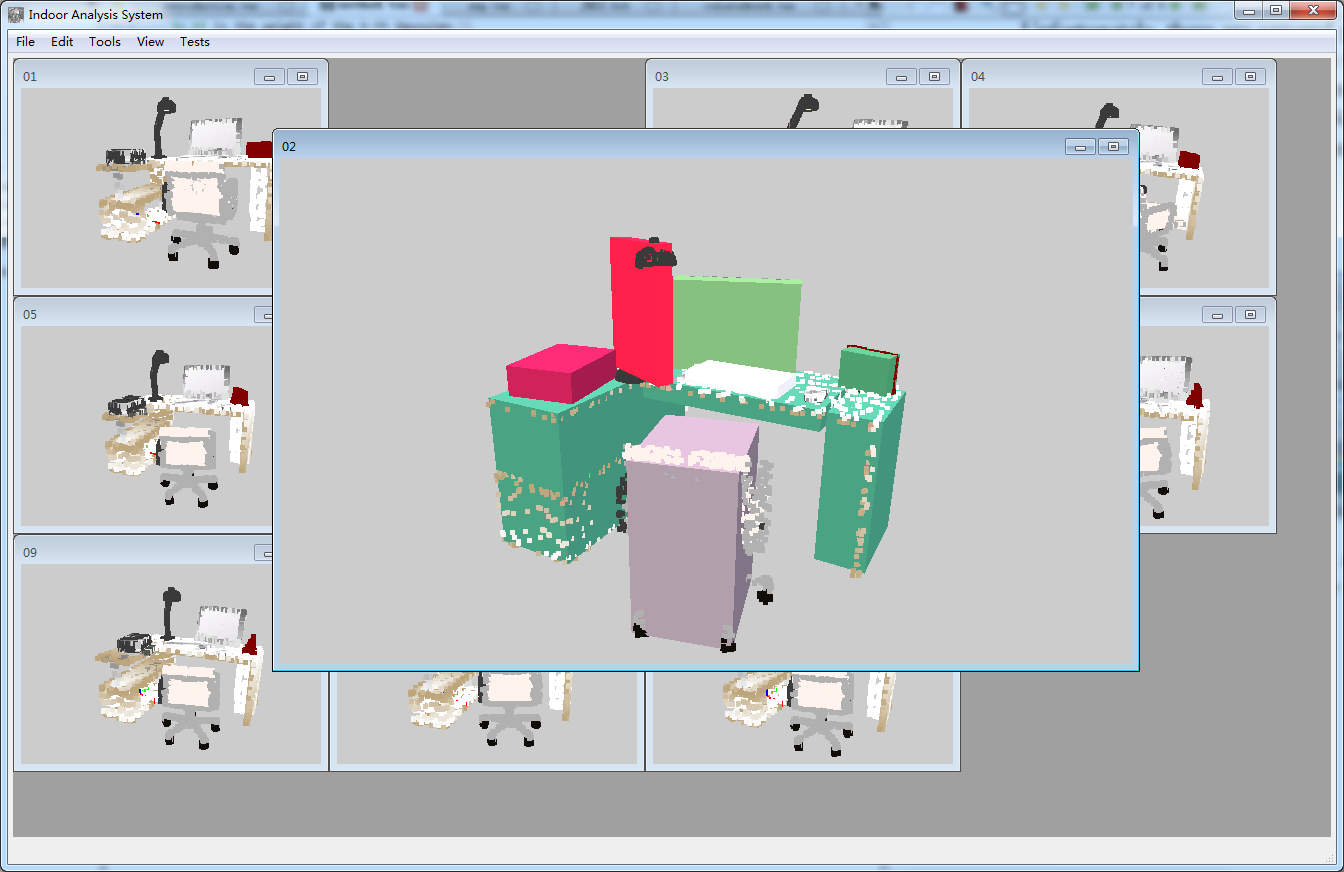
\includegraphics[width=.3\linewidth]{images/interact05.png}
	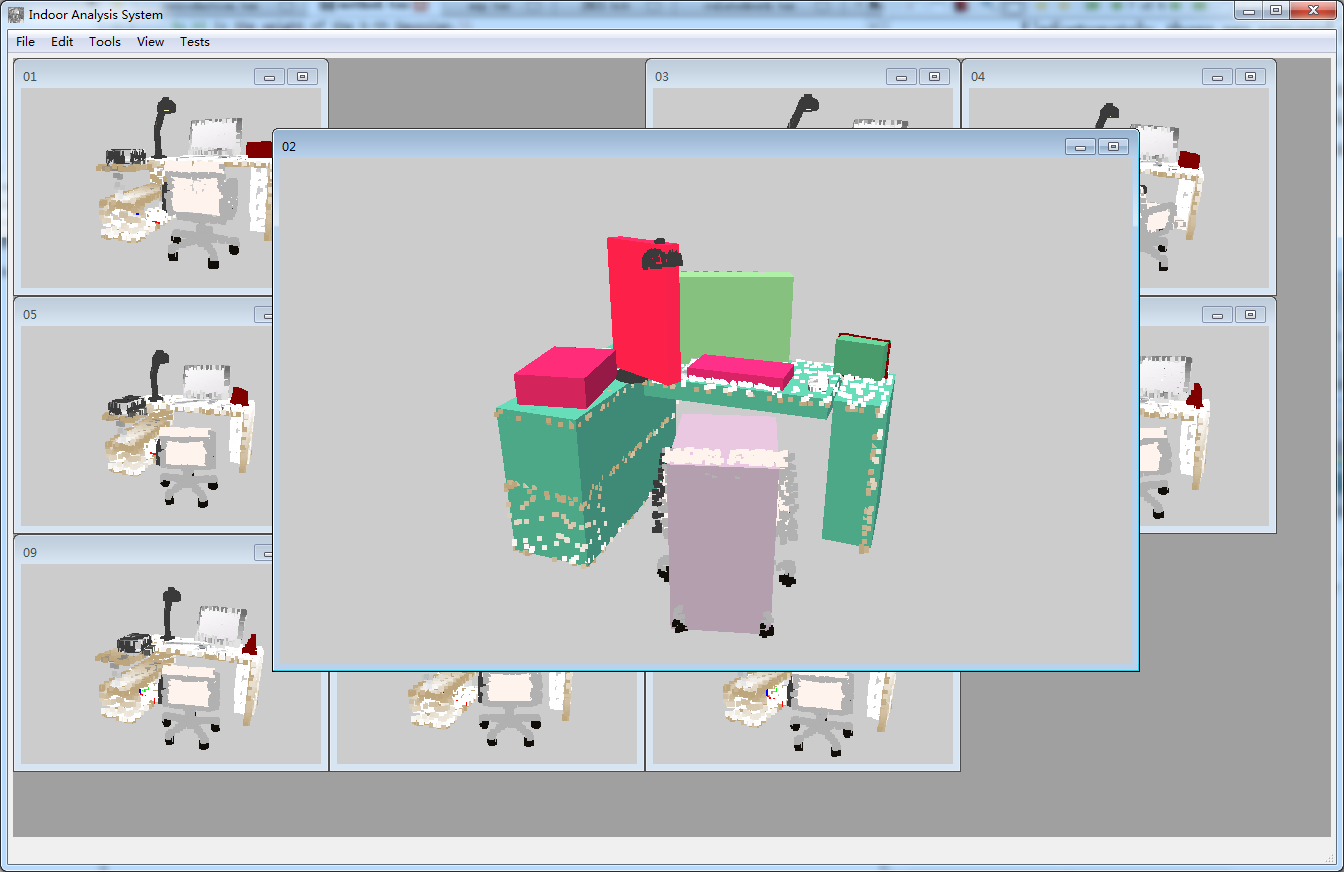
\includegraphics[width=.3\linewidth]{images/interact06.png}
	\caption{\label{fig:interact}
		From the first to the sixth, the nine images show the procedure of interaction:
		the user pick one point set and place boxes in it to indicate the layout for this point set. The box in white is the box currently under editing. The boxes in other colors are boxes placed to represent object layouts. One color represents one object. The interaction allows multiple boxes to represents same object.(e.g. the desk is represented by three boxes in same color)}
\end{figure}

\noindent\textbf{Gaussian Parameters $\{p_k,\mathbf{x}_k,\Sigma_k\}_{k=1}^{K_{all}}$:}
We then set $p_k=\frac{1}{K_{all}}$ as the initial values for $p_k$, which means each Gaussian has the same weight at the beginning. For the Gaussian centroids $\{\mathbf{x}_k\}$, we first allocate memory for total $K_{all}$ Gaussian centroids and then separate them into $N$ groups to represent $N$ objects. Each group has $K_n$ Gaussian centroids based on Eq.~(\ref{equ:K_n}). We implement this by recording the start and end indices of the $N$ objects. In other words, we record $\{0,K_1,K_1+1,K_1+K_2,...,K_S+1,K_S+K_n,...\}$. We initialize the $\{\mathbf{x}_k\}_{K_S+1}^{K_S+K_n}$ for the $n^{th}$ Gaussian group as random positions uniformly distributed on the surface of a sphere, whose radius $r$ is chosen as the median of the radius of the input point sets. 
%
The center of the $n^{th}$ sphere is $\mathbf{c}_n=(0,0,z_n)$, where $z_n\in \{-(N-1)r,-(N-3)r,...,(N-1)r\}$.
%
This means that the object models are vertically arranged in latent space as shown in Figure~\ref{fig:teaser}(c). 
We choose vertical arrangement for groups of object merely for the convenience of visualization.
In the $4^{th}$ row $2^{nd}$ column of Figure~\ref{fig:iter}, an example is shown for the initialization of the Gaussian centroids.
%
The variance $\{\Sigma_k\}$ are all initialized as $\Sigma_k=\sigma^2 I$ in which $\sigma=r$.
The $r$ here is the radius of sphere. Without any prior knowledge, such initialization for Gaussian parameters put all the objects at similar starting condition and they can compete fairly to segment the points in point sets.   

\noindent\textbf{Transformations$\{\phi_{mn}\}_{m=1,n=1}^{M,N}=\{\mathbf{R}_{mn},\mathbf{t}_{mn}\}_{m=1,n=1}^{M,N}$}
Since we have chosen spheres as the initial shapes, we can initialize all the $\mathbf{R}_{mn}$ to identity matrix. For sphere, the different initial orientation makes little differences.
%
For the $\mathbf{t}_{mn}$ we initialize them as $\mathbf{t}_{mn}=- \mathbf{c}_n$ so that all the object model starting with position at origin point when they are transformed to the space of each input set. 
\begin{figure}
	\centering
	\includegraphics[width=\linewidth]{images/localoptimal/localoptimal}
	\caption{\label{fig:localoptimal}This figure shows an example result when converges to a local optimal. (a) is the result of segmentation of this local optimal. (b) is the final centroids of latent model. It shows that from top to down the 2nd and 3rd object model both include part of the table and part of the chair.}
\end{figure}
However, if the $m^{th}$ input point set has the manually placed layout, we treat the associated $\mathbf{t}_{mn}$ differently. For this case we have:
\begin{equation}
	\label{equ:initt}
	\vb{t}_{mn}=\frac{\sum_{\vb{v}_{mi} \in B_n}\vb{v}_{mi}}{N(B_n)}-\vb{c}_n
\end{equation}
where $N(B_n)$ here is the number of element in $B_n$ and $B_n$ is the point set that is enclosed by the manually input layout (boxes) indicating arrangement of the $n^{th}$ object.
\subsection{Layout Constrained Optimization}
The expectation maximization framework is easily converged to a local optimal. To cope with this problem we further use this layout (boxes) from interaction as a soft constraint to guide the optimization and constrain the shape of generated object model. Such constraint is enforced by simply altering the posterior probability $\alpha_{mik}$ as
\begin{equation}
	\label{equ:alteralpha}
	\alpha_{mik}^*=\frac{\alpha_{mik}\beta_{mik}}{\sum_{i,k}\alpha_{mik}\beta_{mik}}
\end{equation}
where the $\beta_{mik}$ is the prior probability according to the boxes. It is defined as:
\begin{equation}
	\beta_{mik}=\left\{
	\begin{array}{rcl}
		1& &\mathbf v_{mi} \in B_n\\
		\exp(-\frac{\min_{\mathbf v_{mj}}|| \mathbf v_{mi} - \mathbf v_{mj} ||_2^2  )}{L})& &\mathbf v_{mi} \notin B_n~and~\mathbf v_{mj} \in B_n\\
	\end{array} \right.
\end{equation}
where the $B_n$ is a point set that is enclosed by the boxes used to represent the layout of $n^{th}$ object. The $k^{th}$ Gaussian model is predefined to be one of the Gaussians used to represent $n^{th}$ object. $\min_{v_{mj}}|| v_{mi} - v_{mj} ||_2^2$ is actually the squared euclidean distance from point $v_{mi}$ to the point set $B_n$, as we define the distance from a point to a point set as the minimum distance from the point to any point inside the point set. $L$ here is a constant number with $L=2r^2$, and $r$ is the median of the radius of input point sets. The radius of a point set is half of length of diagonal line of its axis-aligned bounding box.   
\begin{figure}
	\centering
	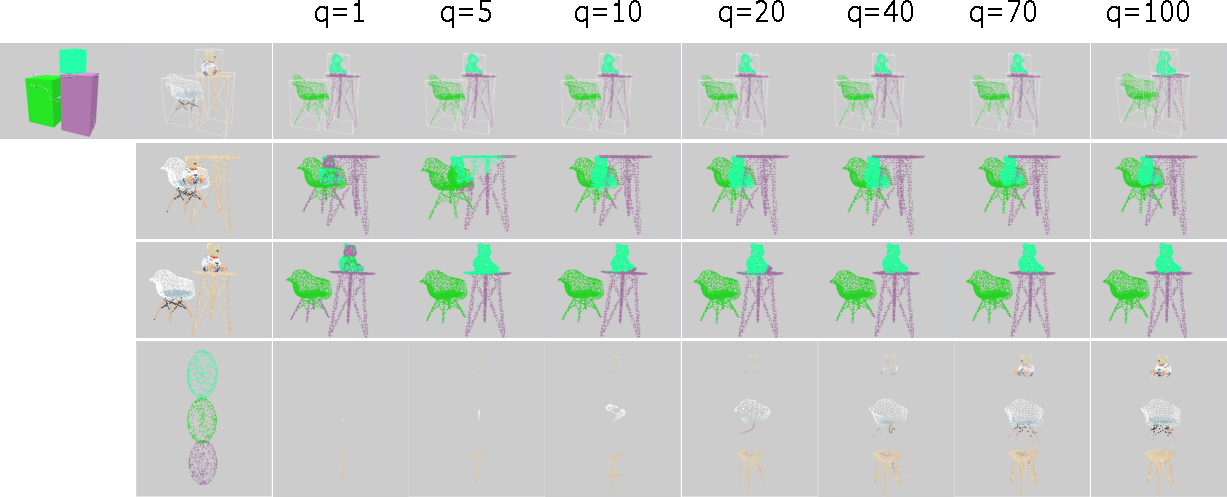
\includegraphics[width=\linewidth]{images/Initialization/iters}
	\caption{\label{fig:iter}This figure shows an example of our algorithm converging with increasing number of iterations. The $1^{st}-3^{rd}$ row show the images for three example out of total nine point sets. The $4^{th}$ row shows the images for Gaussian centroids (the space of object models). The first column shows the input layout (boxes) which is only placed in the first point set. The second column shows the input point sets and the initial Gaussian centroids. The $3^{rd}-9^{th}$ shows result of segmentation (in $1^{st}-3^{rd}$ row) and Gaussian centroids (in $4^{th}$ row) at different iteration numbers $q$. The $q$ is shown at top of each column}
\end{figure}
This alteration on posterior probability is only done with the probability related to the $m^{th}$ point set that have the mannual input layout (the boxes) in it. This alteration can help prevent the object from deforming into an arbitrary shape as shown in Figure~\ref{fig:localoptimal}. In Figure~\ref{fig:localoptimal}, the $2nd$ and $3rd$ object has deformed into a combination of two objects due to lack of constraint.
\begin{figure}
	\centering
	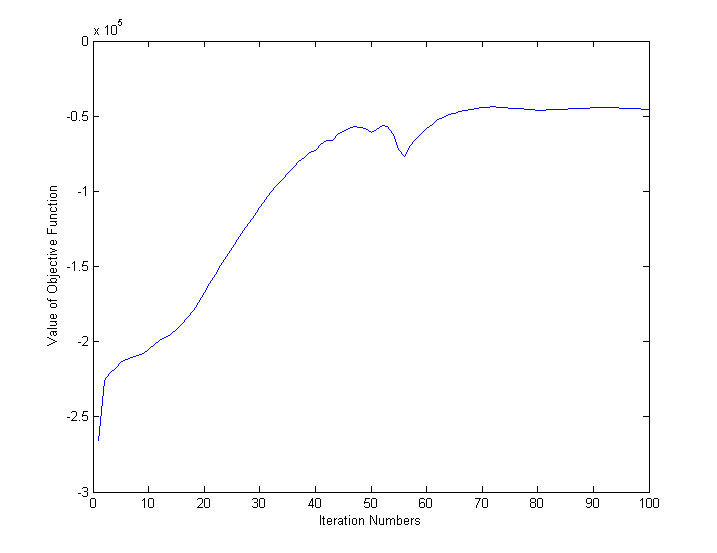
\includegraphics[width=\linewidth]{images/Initialization/obj_iter.png}
	\caption{\label{fig:iter_curve}This figure shows the curve of objective function - iteration number for the data partially shown in Figure~\ref{fig:iter}. The objective value is calculated according to (\ref{equ:obj3}). Note that the curve is not monotonic increasing, which makes it difficult to set a stop condition based on our objective.}
\end{figure}

The Figure~\ref{fig:iter} and Figure~\ref{fig:iter_curve}  shows an example of converging procedure of our algorithm. We want to stress that in the Figure~\ref{fig:iter_curve} the objective function is not monotonic increasing. This is due to our alteration on the posterior probability in (\ref{equ:alteralpha}). This alteration is a quite brutal solution to enforce the shape constraint and it will interfere with the convergence of EM. This makes it difficult for us to set a stop condition for iteration based on objective value. We now stop the iteration when maximum iteration $q_{max}$ is reached as shown in Algorithm~\ref{alg:jrcs} step 8. From the Figure~\ref{fig:iter}, please note that segmentation in the first point set is almost not changed until the last few iterations. This is due to the alteration in (\ref{equ:alteralpha}) as well. In order to constrain the object shape, we do alteration on the posterior probability of first point set based on the boxes in it. This alteration is only done in $q_{alt}$ iterations as shown in Algorithm~\ref{alg:jrcs} step 4. However, the initial segmentation based on mannually input boxes is not accurate. Therefore, we no longer do such alteration in the last few iterations and let the algorithm to refine the segmentation in first point set based on the result of registration. For result in this paper we set $q_{alt}=q_{max}-10$.

For initialization and object shape constraint, we only need the user to input layout ( the boxes ) in one point set. However, in more chanllenging cases our algorithm will stuck at local minimum due to objects' non-local movement. For such cases, our implementation allow the user to add more layouts for other point sets (even during optimization ) and the program can do the same alteration as (\ref{equ:alteralpha}) to further constrain the optimization. We will discuss an example of such case later in Sec~\ref{subsec:interact}.